% appendix: execution microstructure. Blocks moved intact for the 9-page
% NeurIPS main-text boundary (2026-07-19): Methods strategy-lab execution
% and audit paragraphs, Methods flip-risk block, Results stake-sweep
% sentence + figure, Discussion "The two test losses" subsection.
\section{Execution microstructure and the harness audit}
\label{app:execution}

\subsection{The deployed rule}
\label{app:execution_rule}

The deployed rule is seven steps:
\begin{enumerate}
  \item at 00:05, run the Group-A briefing;
  \item re-fuse the voices at every checkpoint and event trigger;
  \item enter at the first hour in 4--9 with edge $\ge 5$ cents,
    traded-side probability $\ge 0.70$ and price $\le 95$ cents, as an
    immediate taker;
  \item stake $\min(\mbox{half balance}, \$400, 1\%\ \mbox{of day
    volume})$, and skip days below \$1k volume;
  \item at 08:35 and 9:00, run position monitors: sell if the traded
    side's fused probability drops below 0.5, flip if the other side
    fully qualifies;
  \item at 9:28, re-check against live futures: enter remaining edges
    $\ge 3$ cents, sell-and-flip on contradiction (the replica replaces
    this voice when live);
  \item at 9:30, log fills against the resolution and refit monthly,
    walk-forward.
\end{enumerate}

\subsection{Modeled execution}
\label{app:execution_model}

Execution is modeled, not assumed. Polymarket's Fee Structure V2,
effective March 30, 2026, makes makers free with a 25\% rebate and charges
takers
\begin{equation}
f = n \, r \, p\,(1-p), \qquad r = 0.04,
\label{eq:takerfee}
\end{equation}

\begin{center}
\small
\begin{tabular}{ll}
\toprule
Symbol & Meaning \\
\midrule
$f$ & taker fee in USDC \\
$n$ & shares filled \\
$r$ & fee rate of the Finance category \\
$p$ & price of the traded side, in USDC \\
\bottomrule
\end{tabular}
\end{center}

which peaks at even odds, about \$1 per 100 shares
\citep{polymarket2026orders}. The entire test half is fee-era,
a built-in regime stress. From roughly 3,400 real trade prints across six
days we calibrated an effective half-spread of about 1 cent and a price
impact of about 0.05 cents per \$100 of stake; the binding constraint is
depth, not slope. Maker fills are modeled pessimistically: the price must
trade through the limit.

An independent audit of the harness found four defects, and all four were
fixed before any conclusion was drawn: fictional fills on zero-volume days
(one such fill carried 46\% of an early result's profit), an entry gate
that admitted bets against the model's own view, over-optimistic maker
fills, and look-ahead in the news-overlay constants, which were refit on
disjoint data. In a thin market, execution assumptions are as load-bearing
as the signal.

\subsection{Flip risk for open positions}
\label{app:execution_flip}

For open positions we also score the risk that the effective gap changes
sign before 9:30. The center drifts about $0.014\%$ per square-root minute,
so
\begin{equation}
P(\mathrm{flip}) = \Phi\!\left(\frac{-\,\lvert 0.83\,g\rvert}
{0.014\%\,\sqrt{\tau}}\right).
\label{eq:flip}
\end{equation}

\begin{center}
\small
\begin{tabular}{ll}
\toprule
Symbol & Meaning \\
\midrule
$g$ & current futures gap, in \% of prior close \\
$0.83$ & effective pass-through used in the drift model \\
$0.014\%$ & fitted drift of the center per $\sqrt{\text{minute}}$ \\
$\tau$ & minutes remaining before 9:30~ET \\
\bottomrule
\end{tabular}
\end{center}

The scale matters more than the formula. A $+0.40\%$ gap at 7:00 carries
about 1\% flip risk; a $+0.10\%$ gap at the same hour carries about 30\%.

\subsection{Stake economics}
\label{app:execution_stakes}

Figure~\ref{fig:stake_sweep} sweeps flat stakes to \$2{,}000:
ROI per dollar is flat at 15.5--16\% from \$25 to \$300, the simulation
leaves its validated calibration region above roughly \$400, and doubling
the intended stake from \$1{,}000 to \$2{,}000 adds only about 27\% more
profit.

\begin{figure}[htp]
    \centering
    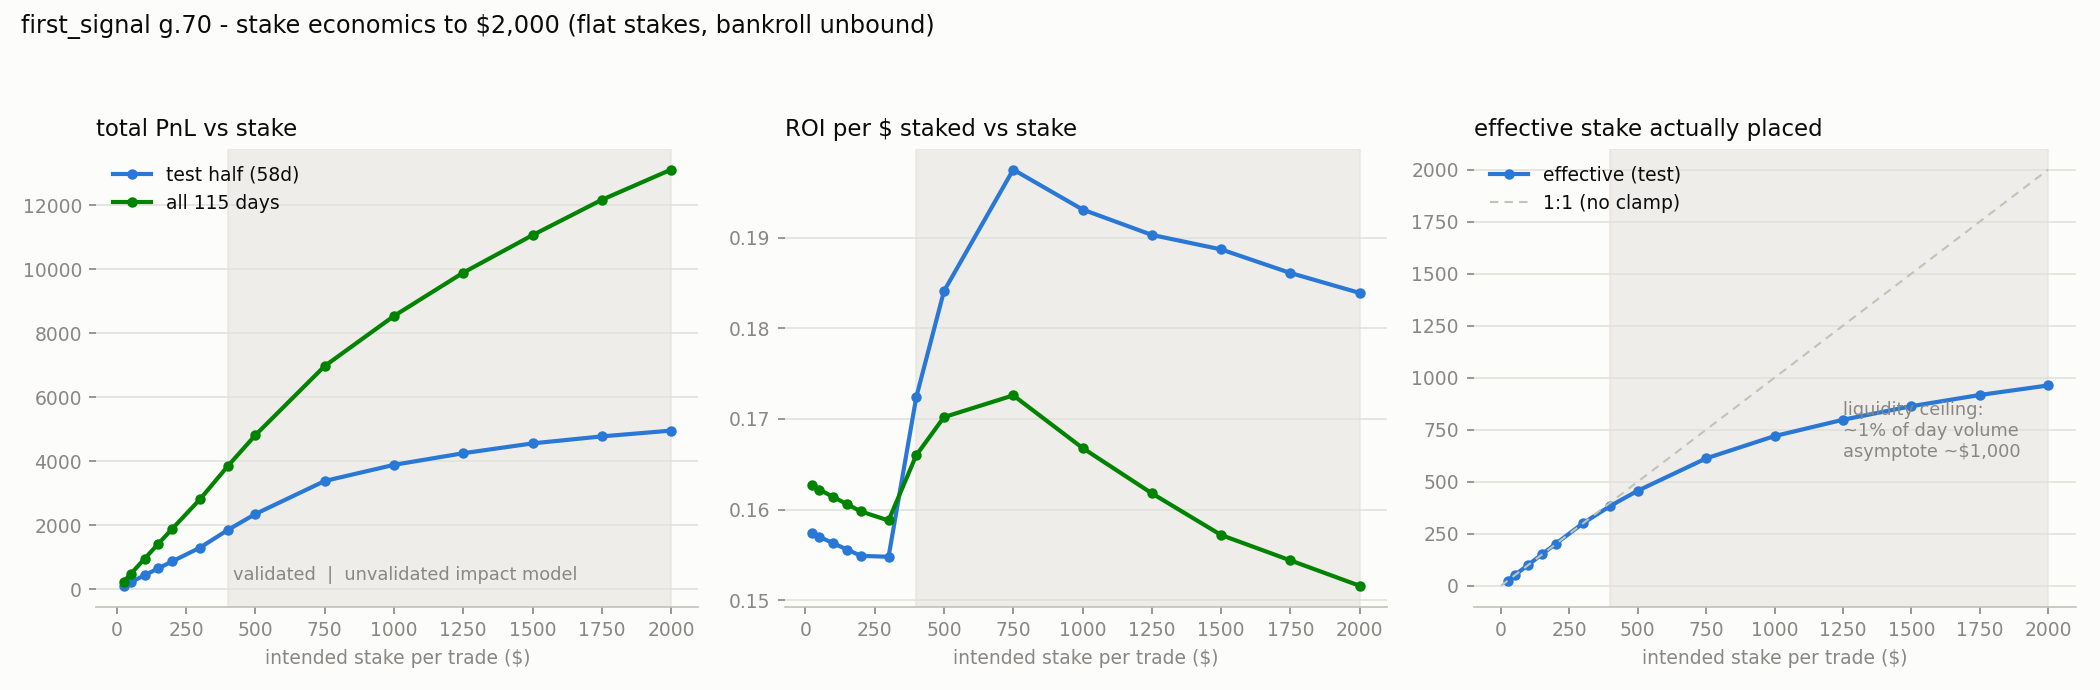
\includegraphics[width=0.92\linewidth]{figures/stake_sweep.png}
    \caption{Stake economics for the first-signal rule (0.70 gate): flat
    stakes swept from \$25 to \$2{,}000 under the calibrated execution
    model, bankroll unbound. Left: total PnL decelerates with stake. Middle:
    ROI per dollar staked is flat near 15.5\% from \$25 to \$300. Right: the
    effective stake bends away from the 1:1 line and asymptotes toward
    roughly \$1{,}000, the 1\%-of-day-volume liquidity ceiling. The shaded
    region above about \$400 marks extrapolation beyond the validated
    \$100--500 calibration range.}
    \label{fig:stake_sweep}
\end{figure}

\subsection{Small verified additions}
\label{app:execution_additions}

The rest of the edge sits in small, verified additions. Position monitors at
08:35 and 9:00, selling if the traded side's fused probability drops below
0.5 and flipping if the other side fully qualifies, added \$43 on train and edge
the champion on test, \$323.67 against \$321.53. A 9:28--9:29 live-futures
leg, scored as $\Phi(0.79\,g / 0.083\%)$ with $g$ the live one-minute
futures gap (Equation~\ref{eq:core} at its 9:29 constants), called the
official open 13 of 13 (95\% CI 77--100) on the only 13 days with minute-level
history and made $+\$107.35$ on three \$50 entries; it cannot be backtested
further and runs paper-first, and the true auction quirks (Jun 1, Jun 22)
stay invisible to it. The strategy is also mostly not trading: it sat out 37
of 58 test days, 30 of which never reach 70\% confidence with a 5-cent edge
at any hour, and trading those days anyway at a 0.60 gate went to ruin. Most
entries are 72--95-cent favorites paying \$4--25 per win; the signature
trade is Jul 14, UP at 49 cents, $+\$50.92$ on a \$50 stake, which alone
paid for both losses.

\subsection{The two test losses}
\label{app:execution_losses}

Both test losses are fully attributed, and they are different kinds of
loss. Jul 2 was a news reversal: a 4:00 DOWN entry at 67.5 cents with an
up-probability of 0.19, then an 8:30 release that blew the gap to
$+0.27\%$. The model reached 0.97 only at 9:00, and by 8:29 the market
already stood at 0.835. About \$77 of the \$296 loss was recoverable at
8:29, and nothing later.

Jul 10 is the more instructive day. We had classified it as an unknowable
auction quirk. It was in fact a late futures flip, the gap moving from
$-0.03\%$ at 9:00 to $+0.08\%$ at 9:29 while the book lagged at
0.715/0.53. A sell-and-flip in the 8:29--9:28 window turns the $-\$307$
loss into $+\$347$, a \$654 swing, with futures data alone. That
reclassification is why the deployed rule carries position monitors and a
9:28 futures leg.
